\documentclass[border=10pt]{standalone}
\usepackage[T1]{fontenc}
\usepackage{tikz}
\usepackage[svgnames]{xcolor}
\usetikzlibrary{shapes.geometric, arrows.meta, positioning, calc}

\colorlet{OrangeFill}{LightSalmon}
\colorlet{OrangeLine}{DarkSalmon!30!Chocolate}
\colorlet{GreenFill}{MediumAquamarine}
\colorlet{GreenLine}{MediumAquamarine!30!Teal}
\colorlet{PurpleFill}{MediumPurple}
\colorlet{PurpleLine}{MediumPurple!30!SlateBlue}
\colorlet{PinkFill}{Thistle}
\colorlet{PinkLine}{Thistle!30!Plum}
\colorlet{BlueFill}{LightSkyBlue}
\colorlet{BlueLine}{SteelBlue}
\colorlet{GrayFill}{LightGray!60!OldLace}
\colorlet{GrayLine}{RosyBrown!50!Silver}

\begin{document}
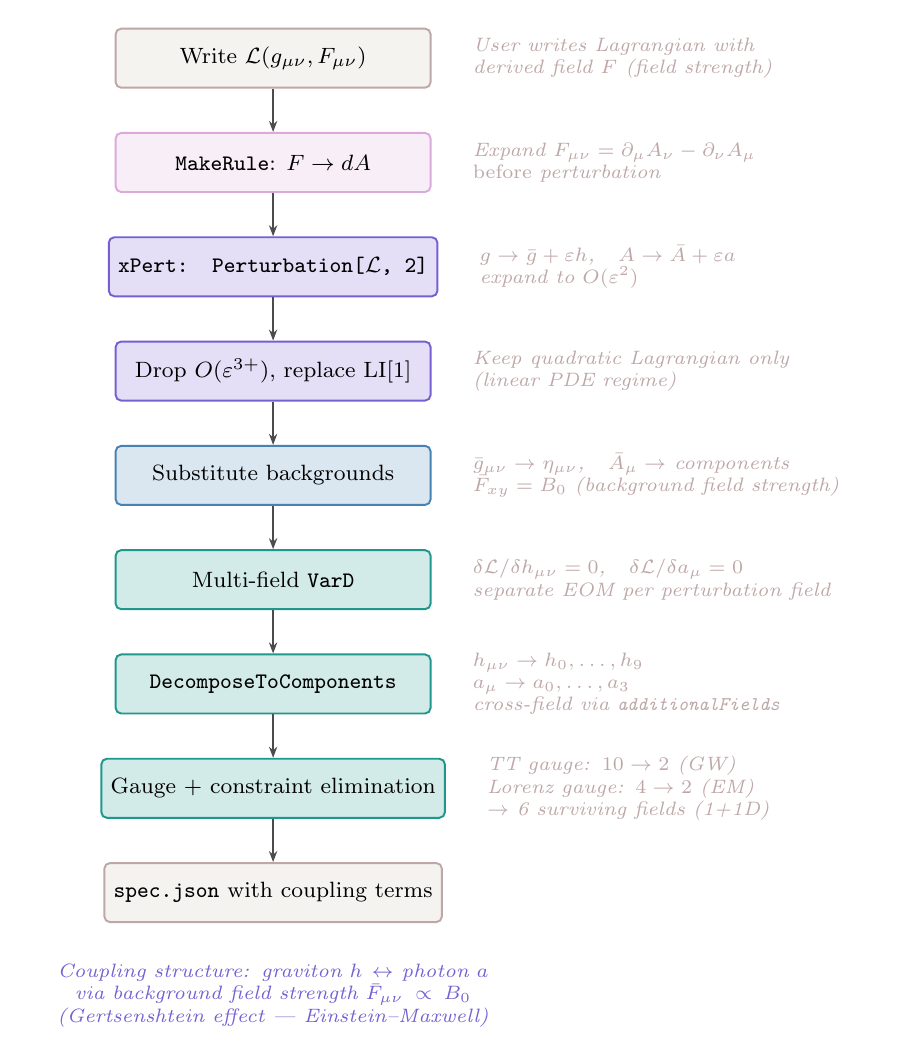
\begin{tikzpicture}[
    stage/.style={
        rectangle, rounded corners=2pt, minimum width=4.0cm,
        minimum height=0.75cm, draw=#1, line width=0.7pt,
        fill=#1!20, font=\footnotesize, align=center,
        text opacity=1, text=black
    },
    stage/.default={black!70},
    annot/.style={font=\scriptsize\itshape, text=GrayLine, align=left,
                  text width=4.8cm},
    arr/.style={-{Stealth[length=4pt, width=3pt]}, semithick, black!70},
    node distance=0.55cm
]

% ===================================================================
% PIPELINE
% ===================================================================

\node[stage=GrayLine, fill=GrayFill, fill opacity=0.4] (lagr)
    {Write $\mathcal{L}(g_{\mu\nu}, F_{\mu\nu})$};
\node[annot, right=0.4cm of lagr.east, anchor=west]
    {User writes Lagrangian with\\derived field $F$ (field strength)};

\node[stage=PinkLine, below=of lagr] (makerule)
    {\texttt{MakeRule}: $F \to dA$};
\node[annot, right=0.4cm of makerule.east, anchor=west]
    {Expand $F_{\mu\nu} = \partial_\mu A_\nu - \partial_\nu A_\mu$\\
     \emph{before} perturbation};

\node[stage=PurpleLine, below=of makerule] (xpert)
    {\texttt{xPert: Perturbation[$\mathcal{L}$, 2]}};
\node[annot, right=0.4cm of xpert.east, anchor=west]
    {$g \to \bar{g} + \varepsilon h$,\quad
     $A \to \bar{A} + \varepsilon a$\\
     expand to $O(\varepsilon^2)$};

\node[stage=PurpleLine, below=of xpert] (truncate)
    {Drop $O(\varepsilon^{3+})$, replace $\mathrm{LI}[1]$};
\node[annot, right=0.4cm of truncate.east, anchor=west]
    {Keep quadratic Lagrangian only\\
     (linear PDE regime)};

\node[stage=BlueLine, below=of truncate] (background)
    {Substitute backgrounds};
\node[annot, right=0.4cm of background.east, anchor=west]
    {$\bar{g}_{\mu\nu} \to \eta_{\mu\nu}$,\quad
     $\bar{A}_\mu \to$ components\\
     $\bar{F}_{xy} = B_0$ (background field strength)};

\node[stage=GreenLine, below=of background] (vard)
    {Multi-field \texttt{VarD}};
\node[annot, right=0.4cm of vard.east, anchor=west]
    {$\delta\mathcal{L}/\delta h_{\mu\nu} = 0$,\quad
     $\delta\mathcal{L}/\delta a_\mu = 0$\\
     separate EOM per perturbation field};

\node[stage=GreenLine, below=of vard] (decompose)
    {\texttt{DecomposeToComponents}};
\node[annot, right=0.4cm of decompose.east, anchor=west]
    {$h_{\mu\nu} \to h_0, \ldots, h_9$\\
     $a_\mu \to a_0, \ldots, a_3$\\
     cross-field via \texttt{additionalFields}};

\node[stage=GreenLine, below=of decompose] (elim)
    {Gauge + constraint elimination};
\node[annot, right=0.4cm of elim.east, anchor=west]
    {TT gauge: $10 \to 2$ (GW)\\
     Lorenz gauge: $4 \to 2$ (EM)\\
     $\to$ 6 surviving fields (1+1D)};

\node[stage=GrayLine, fill=GrayFill, fill opacity=0.4, below=of elim] (json)
    {\textbf{\texttt{spec.json}} with coupling terms};

% ===================================================================
% ARROWS
% ===================================================================
\foreach \a/\b in {lagr/makerule, makerule/xpert, xpert/truncate,
                   truncate/background, background/vard, vard/decompose,
                   decompose/elim, elim/json} {
    \draw[arr] (\a) -- (\b);
}

% ===================================================================
% COUPLING ANNOTATION
% ===================================================================
\node[below=0.4cm of json, font=\scriptsize\itshape, text=PurpleLine,
      align=center, text width=6.0cm] {%
    Coupling structure: graviton $h \leftrightarrow$ photon $a$\\
    via background field strength $\bar{F}_{\mu\nu} \propto B_0$\\
    (Gertsenshtein effect --- Einstein--Maxwell)};

\end{tikzpicture}
\end{document}
